\chapter{Utility, harm and the tolerance they imply}\label{ch:tolerance}

When an institution first writes down a tolerance, it usually writes one. The same
figure is applied to the quarterly series, the research extract and the public
file, and the case for doing so is a serious one. A single tolerance treats every
data subject alike: nobody's confidentiality is worth less because the release that
contains them happens to be more useful. It is simple to explain to a board and to
the public. It leaves no room for an analyst to argue a release through by finding
a reason why this one is special. And it avoids the appearance, which a
confidentiality office has every reason to fear, of trading people's privacy for
the convenience of users. On this view, varying the tolerance from one release to
the next is a step towards negotiating it.

The first fact against the view comes from the shape of the trade-off itself. On
the simulated population of this book, 45 protection settings were assessed, and 11
of them are not dominated by another setting that is both safer and more useful.
Along those 11, the utility gained per unit of added risk runs from 6.0 at the safe
end down to 0.006 at the other.
% source: paper/generated/numbers.tex (\runfrontierpoints 11, \runfrontierslopehigh 6.0, \runfrontierslopelow 0.006); paper/bis_ifc_full.tex, Section sec:sim (45 settings)
A thousandfold difference in the rate of exchange between harm and use means that
one tolerance, applied to releases whose trade-offs differ, buys protection at very
different prices in different places. Where protection is cheap the institution
buys too little of it, and where it is dear it buys too much. The proposition and
corollary below make this exact: a common tolerance is the best choice only in the
special case where every release faces the same trade-off at that tolerance, and
otherwise some other set of tolerances protects as well and serves users better.

The question was faced at national scale before it reached any central bank's
release committee. \citet{abowd2019} argued that the level of protection a
statistical agency gives is a social choice, to be made by weighing the accuracy
of published statistics against the privacy of respondents, at the point where the
rate at which the technology trades one for the other equals the rate at which
society values them. The United States Census Bureau then had to make such a choice
for its 2020 products. Its disclosure avoidance system spent a stated total
privacy-loss budget and divided it among geographic levels and tables
\citep{abowd2022}, and economists who use federal statistics argued in reply that
the accuracy lost had been given too little weight \citep{hotz2022}. Whatever one
thinks of the outcome, the dispute was conducted in the right terms: how much harm
was being prevented, how much use was being given up, and who had the authority to
weigh the two.

At the Bank, the chair was asked to sign a tolerance of 0.12 for every product
drawn from the credit register, and asked Naledi whether that was the right number.
Naledi had no way to answer from the risk tables alone. What she could do was show
the chair what each candidate tolerance would cost each product.

This chapter answers one question. Once an institution states how much weight it
puts on a harm against the use of a release, what tolerance does that weight imply
for each release, and how should a tolerance for a whole programme be shared among
its releases?

\section{Utility and the frontier}\label{c08:sec-frontier}

Utility needs the same discipline as risk. Let $Q$ be a quantity users want to
estimate from the confidential data, and $\widehat{Q}(Y_\theta)$ its estimate from
a release produced under protection setting $\theta$. A loss-based utility is
\begin{equation}\label{c08:eq-util}
U(\theta) = -\E\big[\mathcal{L}\{\widehat{Q}(Y_\theta),\ Q\}\big],
\end{equation}
where the expectation runs over sampling and the randomness of the mechanism, and
the loss $\mathcal{L}$ is declared before any setting is evaluated. Squared error,
the distortion of a confidence interval, or a weighted loss over the analyses users
are known to run are all admissible \citep{karr2006,snoke2018}. The loss must be
declared in advance for the same reason the adversary must: a setting chosen after
seeing which loss it happens to do well on carries no guarantee.

For each setting, the institution now has two numbers: a risk coordinate and a
utility. Following the decision rule of Chapter~\ref{ch:thresholds}, the risk
coordinate should be the upper bound $\overline{R}_{1-\alpha}(\theta)$ that the
release decision will use, not the point estimate. The attainable set is
\[
\mathcal{A} = \{(\overline{R}_{1-\alpha}(\theta),\ U(\theta)) : \theta \in \Theta\} .
\]
A point is dominated if another attainable point has no more risk and no less
utility, with one of the two strict. The \emph{risk--utility frontier} $\mathcal{F}$
is the set of points that are not dominated, the confidentiality map of
\citet{duncan2001} drawn with a bound on the risk axis. No sensible institution
chooses a dominated setting, so every choice worth discussing lies on the frontier,
and the discussion is about where on it to stand.

Figure~\ref{c08:fig-frontier} shows the frontier for the simulated population. The
45 settings vary the width of age bands, the number of occupation groups and the
minimum cell count. The frontier spans risk bounds from 0.081 to 0.564, and it is
steep at the safe end: halving the bound from 0.1715 to 0.0806 costs 0.17 of
utility, half the range the frontier spans, and cuts the records kept from all of
them to 58 per cent.
% source: paper/generated/numbers.tex (\runfrontierrisklow 0.081, \runfrontierriskhigh 0.564); paper/bis_ifc_full.tex, Section sec:sim ("halving the bound from 0.1715 to 0.0806 costs 0.17 of utility ... from 100 to 58 per cent")
A committee looking at the figure can see at once what it is being asked to trade.

\begin{figure}[ht]
\centering
\includegraphics[width=0.72\textwidth]{fig2_frontier.pdf}
\caption{Risk and utility for 45 protection settings on the simulated population.
The risk coordinate is the one-sided 95 per cent upper bound for a uniformly drawn
target, not the point estimate. Squares mark the setting that maximises value for
three values of the relative harm weight $\kappa$; the risk of each is the implied
tolerance of Proposition~\ref{c08:prop-tau}.}
\label{c08:fig-frontier}
\end{figure}

Two cautions come with the picture. The frontier is estimated, and using the upper
bound as the risk coordinate moves every point to the right by an amount that
shrinks as the number of simulated attacks grows. A frontier drawn with point
estimates and a decision rule applied with bounds are different objects, and an
institution that mixes them will choose settings that its own rule then rejects.
Second, the frontier of a real mechanism family is a set of points, not a curve.
Its slopes on the simulated population fall from 6.0 to 0.006 but not steadily, so
the frontier is not concave, which is what a family of discrete settings produces.
% source: paper/generated/numbers.tex (\runfrontierslopehigh, \runfrontierslopelow); paper/bis_ifc_full.tex, Section sec:sim ("not monotonically")
The propositions below are stated for a smooth concave frontier, where they are
cleanest, and Section~\ref{c08:sec-discrete} gives the discrete version a committee
actually uses.

\section{The tolerance a harm weight implies}\label{c08:sec-implied}

Suppose the institution values one unit of utility at $\lambda > 0$ and one unit of
risk, for the declared harm class, at $c_h > 0$. No monetary valuation is needed;
only the ratio enters,
\[
\kappa = \frac{c_h}{\lambda},
\]
which we call the \emph{relative harm weight}. It is measured in units of utility per
unit of risk: it is the utility gain the institution would require before accepting
one more unit of risk. The value of a setting is
\begin{equation}\label{c08:eq-value}
V(\theta) = \lambda\,U(\theta) - c_h\,\overline{R}_{1-\alpha}(\theta) .
\end{equation}

\begin{proposition}[Implied tolerance]\label{c08:prop-tau}
Let the frontier be the graph of a differentiable, increasing, strictly concave
function $u = \varphi(r)$ on $[\underline{r}, \overline{r}]$. The maximiser of
\eqref{c08:eq-value} over the frontier exists and is unique. If
$\varphi'(\underline{r}) > \kappa > \varphi'(\overline{r})$, it is interior and its
risk $\tau^\star$ satisfies
\begin{equation}\label{c08:eq-tangency}
\varphi'(\tau^\star) = \kappa .
\end{equation}
If $\kappa \ge \varphi'(\underline{r})$ then $\tau^\star = \underline{r}$, and if
$\kappa \le \varphi'(\overline{r})$ then $\tau^\star = \overline{r}$. In every case
$\tau^\star$ is nonincreasing in $\kappa$, and strictly decreasing over the interior
range.
\end{proposition}

The proposition is the disclosure-control counterpart of the social-choice argument
of \citet{abowd2019}, and it has the form of a Bayes decision under a linear loss
\citep{berger1985}. Its practical use is not to compute the tolerance. A harm weight
is no easier to state than a tolerance. Its use is to show that the two are the same
statement made in different units. An institution that adopts a tolerance has, by
\eqref{c08:eq-tangency}, adopted the harm weight equal to the frontier's slope at
that tolerance, whether or not anyone said so. An institution that adopts 0.05 on
one release and 0.20 on another has, in general, put different weights on the same
harm, and it should be able to say why.

Figure~\ref{c08:fig-implied} reads the implied tolerance off the simulated frontier
for six harm weights. At $\kappa = 0.25$ the institution would release the file
without suppression, at a bound of 0.464. At $\kappa = 0.5$ it would coarsen the age
bands and still keep every record, at 0.345. Doubling the weight to 1 cuts the
tolerance to 0.145 and moves the release to three occupation groups with a minimum
cell count of five, keeping 94 per cent of records. At $\kappa = 5$ and above the
tolerance is 0.081 and the minimum cell count is 20, which keeps 58 per cent.
% source: paper/generated/table_tolerance.tex; paper/generated/numbers.tex (\runtolerancekappa025 ... \runtolerancekappa10)

\begin{figure}[ht]
\centering
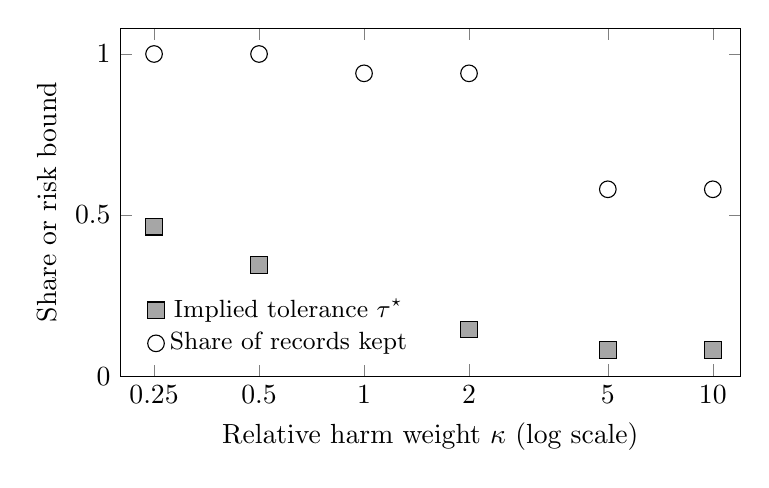
\begin{tikzpicture}
\begin{axis}[
  width=0.78\textwidth, height=6cm, xmode=log,
  xlabel={Relative harm weight $\kappa$ (log scale)},
  ylabel={Share or risk bound},
  xmin=0.2, xmax=12, ymin=0, ymax=1.08,
  xtick={0.25,0.5,1,2,5,10}, xticklabels={0.25,0.5,1,2,5,10},
  legend style={at={(0.03,0.03)},anchor=south west,draw=none,font=\small,fill=white}]
\addplot[black, only marks, mark=square*, mark size=3pt, mark options={fill=gray!70}]
  coordinates {(0.25,0.464) (0.5,0.345) (1,0.145) (2,0.145) (5,0.081) (10,0.081)};
\addplot[black, only marks, mark=o, mark size=3pt]
  coordinates {(0.25,1.00) (0.5,1.00) (1,0.94) (2,0.94) (5,0.58) (10,0.58)};
\legend{Implied tolerance $\tau^\star$, Share of records kept}
\end{axis}
\end{tikzpicture}
% source: paper/generated/table_tolerance.tex
\caption{The tolerance implied by six relative harm weights on the simulated
population (filled grey squares), and the share of records the selected setting
keeps (open white circles). Only these six weights were evaluated; between two
neighbouring weights with different values the setting changes at some point not shown. Each value maximises utility minus
$\kappa$ times the upper risk bound over the 11 settings on the frontier.}
\label{c08:fig-implied}
\end{figure}

Two features of the figure carry over to practice. The implied tolerance is flat
over wide ranges of the weight: one setting is best for every weight from 5 to 10.
And it jumps between ranges: between weights of 0.5 and 1, a modest change in how
much the institution cares about the harm moves the release from an unsuppressed
file with twelve occupation groups to a suppressed file with three. The jumps come
from the discrete family of settings, not from the argument. They mean that over
most of the range an institution cannot fine-tune its tolerance, and that near a
breakpoint a small revision of the harm weight changes the product.

The credit register shows how much rides on the choice. At a tolerance of 0.05, an
adversary who holds a single release already requires a floor of 40, and against
the full pooled adversary no floor up to 300 suffices. At 0.20, the three outside
adversaries require floors of 1, 5 and 30.
% source: paper/generated/table_tolerance_floors.tex (selection floors before confirmation)
The floors move by an order of magnitude across a range of tolerances that a
committee might regard as close together, which is why the tolerance deserves the
same scrutiny as the adversary.

When Naledi brought the chair a figure of this kind for the credit register, the
chair did not ask for the tolerance, but asked what each step
down the curve would cost the users of each product, and which harm the step
prevented. That was the right question, and it is the one the rest of this chapter
turns into a procedure.

\section{Why one tolerance for every release is usually inefficient}\label{c08:sec-uniform}

The tangency condition applies release by release. A programme whose releases share
a harm class, and so a harm weight, but face different trade-offs, has a different
implied tolerance for each.

\begin{corollary}[Uniform tolerances are usually inefficient]\label{c08:cor-uniform}
Let releases $i = 1,\dots,m$ have frontiers $\varphi_i$ satisfying the conditions of
Proposition~\ref{c08:prop-tau}, and a common relative harm weight $\kappa$ in the
interior range of each. A common tolerance $\tau$ maximises total value
$\sum_i \{\lambda \varphi_i(\tau_i) - c_h \tau_i\}$ only if $\varphi_i'(\tau) =
\kappa$ for every $i$. Otherwise total value strictly increases when the tolerance
is tightened on releases whose frontier is flat at $\tau$ and loosened on releases
whose frontier is steep there.
\end{corollary}

A frontier is flat at a tolerance when protection is cheap there: a large cut in
risk costs little utility. It is steep when protection is dear. A uniform tolerance
asks every release to stop at the same risk, and so it stops the cheap releases
short of the protection they could give at little cost, and pushes the dear ones
beyond the point where the protection is worth what it destroys. Moving
tolerance from where protection is dear to where it is cheap leaves the institution
better off on both counts it cares about.

The fairness argument for a uniform tolerance deserves a direct reply. Equal
treatment of data subjects is the right principle, but a uniform tolerance across
releases is not what delivers it. The quantity that should be the same for
everyone exposed to the same harm is the weight the institution puts on that harm,
$\kappa$, because that is the statement of how much a person's exposure counts
against the public's use of the data. Applying one weight consistently gives
different tolerances on releases whose trade-offs differ, and that is the
consistent treatment. A uniform tolerance, by contrast, puts different implied
weights on the same harm in different releases, so it is the uniform figure that
treats people unequally, through the back door of the frontier's slope. The
principle also needs the protected parties of Chapter~\ref{ch:thresholds}: a weight
is set per harm class and per party, and a borrower's identification and a lender's
reconstructed position need not carry the same weight. And it needs the programme
view of Chapter~\ref{ch:programmes}, because one person appears in many releases,
and equal per-release tolerances say nothing about the risk to that person once the
releases are pooled.

Two cautions belong with the corollary. The harm weight is not found in the data.
Choosing it is a governance and ethical decision, and no estimation procedure will
supply it. What the corollary does is force the choice into the open, because a
tolerance already implies a weight. The second caution follows from the first. The
owner of the threshold has to be senior enough to state the weight on the
institution's behalf and answer for it in public, which in a central bank means the
release committee or the executive member who chairs it, and not the analyst who
runs the simulation. An owner who cannot defend the weight in public is not the
right owner.

\section{A discrete frontier and a practical way to state a weight}\label{c08:sec-discrete}

Real settings form a finite grid, and Proposition~\ref{c08:prop-tau} needs a
smooth, concave curve. The general existence result covers both.

\begin{proposition}[Existence]\label{c08:prop-exist}
Let $T$ be the declared target set. If $\Theta$ is compact, $U$ is upper
semicontinuous, $\theta \mapsto \max_{t \in T}\overline{R}_{1-\alpha}(t,\theta)$ is
lower semicontinuous, and some setting meets the tolerance $\tau$, then the problem
of maximising $U(\theta)$ subject to
$\max_{t \in T}\overline{R}_{1-\alpha}(t,\theta) \le \tau$ has a solution.
\end{proposition}

On a finite grid every function is continuous in the trivial sense and the maximum
exists, so the result adds nothing there. What a finite grid needs is a statement of
which settings any harm weight could select, and what a chosen setting says about
the weight. Order the frontier points by risk, $(r_1, u_1), \dots, (r_K, u_K)$ with
$r_1 < \dots < r_K$ and therefore $u_1 < \dots < u_K$, and define the trade between
two points $i < j$ as
\[
s_{ij} = \frac{u_j - u_i}{r_j - r_i},
\]
the utility gained per unit of risk added in moving from $i$ to $j$.

\begin{proposition}[What a chosen setting says about the weight]\label{c08:prop-bracket}
Frontier point $j$ maximises $u - \kappa r$ over the frontier if and only if
\begin{equation}\label{c08:eq-bracket}
\max_{i > j} s_{ji} \ \le\ \kappa\ \le\ \min_{i < j} s_{ij},
\end{equation}
with the maximum over an empty set read as $0$ and the minimum over an empty set as
$+\infty$. The set of weights that select $j$ is therefore an interval, and it is
empty exactly when $(r_j, u_j)$ lies below the upper concave hull of the frontier.
\end{proposition}

The proposition gives the committee a procedure that needs no number it cannot
supply. The analyst lists the settings on the upper concave hull of the frontier,
in order of risk. For each neighbouring pair, she writes one line: moving from
setting $A$ to the safer setting $B$ lowers the upper risk bound from $r_A$ to $r_B$,
for the declared adversary and harm, and costs this much utility, described in terms
users recognise, such as the share of records kept, the occupation detail lost or
the error added to a published ratio. The owner answers each line yes or no: is the
reduction in risk worth the loss? Each answer places $\kappa$ above or below one
trade, and because the trades decline along the hull, the answers locate the weight
in one interval and select one setting. On the simulated population the hull has
at most 11 points, so a few questions suffice, and the flat stretches of
Figure~\ref{c08:fig-implied} mean that most of the range of possible weights leads
to the same handful of settings.

The procedure produces three things the record should keep: the questions as put
and the owner's answers, the interval of weights they imply, and the setting
selected. It also catches two errors. A setting that lies below the hull cannot be
selected by any weight, so a proposal to release it is a proposal to accept a
setting that some other setting beats for every view of the harm; the proposition
says so, and the analyst can point to the setting that beats it. And when two
releases of the same harm class and protected party carry weight intervals that do
not overlap, the institution has put different weights on the same harm, and the
record must say why.

When Grace read the records of the Bank's first year under this procedure, she did
exactly that comparison. Two research extracts drawn from the credit register, for
the same harm and the same protected party, had been signed with weight intervals
that did not overlap. The record of the second named a reason: the second extract
went only to a secure environment, under a different access route, with a different
declared adversary. That was a reason the procedure allows. Without it the
difference would have been a finding.

\section{A risk budget across a programme}\label{c08:sec-budget}

A programme raises the question of tolerance in a second form. Suppose an
institution has decided how much risk the whole programme may carry and must divide
it among its releases. Chapter~\ref{ch:programmes} showed that the probability that
at least one release, used alone, exposes a target is at most the sum of the
releases' risks. An institution that governs that union event can therefore impose
$\sum_i r_i \le \tau_{\mathrm{prog}}$ and allocate the budget. Release $i$ has value
weight $w_i > 0$, and for simplicity the releases share one frontier shape
$\varphi$.

\begin{proposition}[Risk budget]\label{c08:prop-budget}
Let $\varphi$ be increasing, differentiable and strictly concave on $(0,\infty)$,
with $\varphi'(0^+) = \infty$. The problem of maximising $\sum_i w_i \varphi(r_i)$
subject to $\sum_i r_i \le \tau_{\mathrm{prog}}$ and $r_i \ge 0$ has a unique
solution, characterised by
\begin{equation}\label{c08:eq-water}
w_i\,\varphi'(r_i^\star) = \mu \quad \text{for every } i, \qquad
\sum_i r_i^\star = \tau_{\mathrm{prog}},
\end{equation}
for some $\mu > 0$. If $\varphi(r) = \log r$, then $r_i^\star = \tau_{\mathrm{prog}}
w_i / \sum_j w_j$. If $\varphi(r) = a + b r^{\gamma}$ with $b < 0$ and $\gamma < 0$,
then $r_i^\star \propto w_i^{1/(1-\gamma)}$.
\end{proposition}

Every release ends with the same weighted marginal value of risk. The equal split,
$r_i = \tau_{\mathrm{prog}}/m$, which is what an institution does by default when it
applies one tolerance to every release, satisfies \eqref{c08:eq-water} only when all
the value weights are equal. The proportional rule is just as particular: it is
right for the logarithmic value curve and for no other. For the power family, the
exponent $1/(1-\gamma)$ is below one when $\gamma < 0$, so the allocation is flatter
than value, and it tends to the equal split as $\gamma \to -\infty$.

The repository fits the power curve to the simulated frontier, with $R^2 = 0.964$
and $\gamma = -0.23$, which gives an exponent of 0.81. For four releases with value
weights 1.0, 0.7, 0.5 and 0.3 and a programme budget of 0.5, the allocation is
0.186, 0.139, 0.106 and 0.070, against 0.125 each under the equal split, and on the
fitted curve it cuts the total loss by 4.5 per cent relative to the equal split.
% source: paper/generated/numbers.tex (\runfrontierfitr2 0.964, \runfrontiergamma -0.23, \runbudgetexponent 0.81, \runbudgetallocation, \runbudgetequalshare 0.125, \runbudgetgain 4.5); weights and budget from configs/paper.json ("programme": weights [1.0, 0.7, 0.5, 0.3], tau_programme 0.5)
Figure~\ref{c08:fig-budget} sets the three rules side by side. The proportional
shares, 0.200, 0.140, 0.100 and 0.060, follow from the same weights and budget.
% source: computed as 0.5 * w_i / sum(w) from configs/paper.json weights, as in privacy_risk.experiments.programme_budget ("proportional")
The figure is a stylised illustration: the frontier it rests on is not concave, the
fitted curve smooths it, and the 4.5 per cent is a gain on the curve, not on the
discrete settings. Its lesson is qualitative. The default rule is optimal only by
coincidence, and the gain from doing better depends on how unequal the releases'
values are and how sharply the frontier bends.

\begin{figure}[ht]
\centering
\begin{tikzpicture}
\begin{axis}[
  ybar, bar width=9pt, width=0.8\textwidth, height=6cm,
  symbolic x coords={R1,R2,R3,R4}, xtick=data,
  xticklabels={{Release 1\\$w=1.0$},{Release 2\\$w=0.7$},{Release 3\\$w=0.5$},{Release 4\\$w=0.3$}},
  xticklabel style={align=center,font=\small},
  ylabel={Share of the programme budget}, ymin=0, ymax=0.23, area legend,
  enlarge x limits=0.18,
  legend style={at={(0.5,1.03)},anchor=south,draw=none,font=\small,legend columns=3,/tikz/every even column/.append style={column sep=6pt}},
  yticklabel style={/pgf/number format/fixed,/pgf/number format/precision=2}]
\addplot[fill=gray!70, draw=black]
  coordinates {(R1,0.186) (R2,0.139) (R3,0.106) (R4,0.070)};
\addplot[fill=white, draw=black, postaction={pattern=north east lines}]
  coordinates {(R1,0.125) (R2,0.125) (R3,0.125) (R4,0.125)};
\addplot[fill=gray!20, draw=black, postaction={pattern=dots}]
  coordinates {(R1,0.200) (R2,0.140) (R3,0.100) (R4,0.060)};
\legend{Optimal on fitted curve, Equal split, Proportional to value}
\end{axis}
\end{tikzpicture}
% source: paper/generated/numbers.tex (\runbudgetallocation, \runbudgetequalshare); configs/paper.json
\caption{Three ways to divide a programme budget of 0.5 among four releases with
value weights 1.0, 0.7, 0.5 and 0.3. Solid dark bars: the allocation that maximises
value on the power curve fitted to the simulated frontier. Hatched white bars: the
equal split. Dotted light bars: shares proportional to value, which would be optimal
for a logarithmic value curve.}
\label{c08:fig-budget}
\end{figure}

The scope of the budget must be stated with it. Proposition~\ref{c08:prop-budget}
governs the union event, the chance that some single release, used alone, exposes
a target. It does not govern an adversary who pools the releases, and
Chapter~\ref{ch:programmes} proved that no statement in terms of the releases'
separate risks can. A risk budget allocates attention and protection across
releases. It does not replace the joint simulation of the pooled attack, and a
record that cites a budget as evidence about pooled risk misstates what the budget
shows. The Census Bureau's division of its privacy-loss budget among geographic
levels differs on exactly this point: a formal privacy accountant composes across
releases without any assumption about how they depend on one another
\citep{dwork2014}, which is the subject of Chapter~10, whereas a budget on the
union of attack events composes only for the event it names.

\section{The answer}\label{c08:sec-answer}

The chapter asked what tolerance a stated harm weight implies for each release, and
how a programme's tolerance should be shared. For each release, the implied
tolerance is the point on its risk--utility frontier where the utility gained per
unit of added risk equals the institution's harm weight; on a discrete frontier it
is the setting whose interval of weights contains the institution's weight. Since
frontiers differ, so do the implied tolerances, and one tolerance for every release
is the right choice only when every frontier has the same slope at it. Fairness is
served by applying one harm weight, per harm class and protected party, to every
release, which gives tolerances that differ. Across a programme governed on the
union event, the budget should be divided so that every release ends with the same
weighted marginal value of risk; the equal split does this only when the releases
are of equal value. In practice a committee need not state a weight as a number. It
answers a short sequence of questions about whether one step down the frontier is
worth its cost, and its answers fix both the weight and the release.

\begin{inpractice}[In practice: setting tolerances across releases]\sloppy
Declare the utility loss for each release before any setting is evaluated, and plot
the frontier with the upper bound the decision will use. Present the owner with the
settings on the upper concave hull, in order of risk, and with one line per
neighbouring pair stating the risk removed and the use lost. Record the owner's
answers, the interval of harm weights they imply and the setting selected. Use one
harm weight per harm class and protected party across releases, and write down the
reason whenever two releases with the same harm and party carry weights that
disagree. When dividing a programme budget, give more to the releases of greater
value, but do not cite the budget as evidence about an adversary who pools the
releases.

\smallskip\noindent\textit{In the software.} \texttt{privacy\_risk.frontier} holds
\texttt{nondominated} for the frontier, \texttt{choose\_max\_utility} for the
constrained choice, \texttt{fit\_value\_curve} for the power curve and
\texttt{concavity\_diagnostic}, which reports the successive slopes and whether they
decline. \texttt{privacy\_risk.governance.implied\_tolerance} returns the setting
that maximises utility minus $\kappa$ times the risk bound, and
\texttt{risk\_budget} and \texttt{budget\_value} implement
Proposition~\ref{c08:prop-budget} for the power curve.
\texttt{privacy\_risk.experiments.programme\_budget} checks the closed form against
a numerical optimum. The interval of Proposition~\ref{c08:prop-bracket} is not yet
implemented; it follows from the slopes that \texttt{concavity\_diagnostic}
returns. The allocation itself is short:
\begin{lstlisting}
exponent = 1.0 / (1.0 - gamma)
shares = weights ** exponent
return programme_tolerance * shares / shares.sum()
\end{lstlisting}
\end{inpractice}

\section{Proofs}\label{c08:sec-proofs}

\begin{proof}[Proof of Proposition~\ref{c08:prop-tau}]
On the frontier the problem is to maximise $J(r) = \lambda\varphi(r) - c_h r$ over
$[\underline{r}, \overline{r}]$. $J$ is continuous on a compact interval, so a
maximiser exists, and it is strictly concave because $\varphi$ is, so the
maximiser is unique. Its derivative $J'(r) = \lambda\{\varphi'(r) - \kappa\}$ is
strictly decreasing. If $\varphi'(\underline{r}) > \kappa > \varphi'(\overline{r})$,
then $J'$ is positive at $\underline{r}$ and negative at $\overline{r}$, so it has a
unique zero in the interior, which is the maximiser and satisfies
\eqref{c08:eq-tangency}. If $\kappa \ge \varphi'(\underline{r})$, then $J'(r) < 0$
for every $r > \underline{r}$, so $J$ is decreasing and the maximiser is
$\underline{r}$. If $\kappa \le \varphi'(\overline{r})$, then $J'(r) > 0$ for every
$r < \overline{r}$, and the maximiser is $\overline{r}$. Over the interior range
$\tau^\star = (\varphi')^{-1}(\kappa)$, and the inverse of a strictly decreasing
function is strictly decreasing. Combining the three ranges, $\tau^\star$ equals
$\overline{r}$ for small $\kappa$, decreases strictly through the interior range,
and equals $\underline{r}$ for large $\kappa$, so it is nonincreasing throughout.
\end{proof}

\begin{proof}[Proof of Corollary~\ref{c08:cor-uniform}]
Total value is a sum of terms each depending on one $\tau_i$, so it is maximised by
maximising each term separately. By Proposition~\ref{c08:prop-tau}, with $\kappa$ in
the interior range of every release, the unique maximiser of term $i$ is the
$\tau_i^\star$ solving $\varphi_i'(\tau_i^\star) = \kappa$. A common tolerance $\tau$
is optimal only if $\tau = \tau_i^\star$ for every $i$, that is
$\varphi_i'(\tau) = \kappa$ for every $i$. If this fails for some $i$, then
$\tau \ne \tau_i^\star$, and by strict concavity term $i$ increases strictly when
$\tau_i$ moves from $\tau$ towards $\tau_i^\star$. When $\varphi_i'(\tau) < \kappa$
the frontier is flat at $\tau$ and $\tau_i^\star < \tau$, so the move tightens the
tolerance; when $\varphi_i'(\tau) > \kappa$ it is steep and $\tau_i^\star > \tau$, so
the move loosens it. The other terms are unchanged, so total value increases
strictly.
\end{proof}

\begin{proof}[Proof of Proposition~\ref{c08:prop-exist}]
The feasible set $\Theta_\tau = \{\theta : \max_{t \in T}
\overline{R}_{1-\alpha}(t,\theta) \le \tau\}$ is a sublevel set of a lower
semicontinuous function, hence closed, and as a closed subset of the compact
$\Theta$ it is compact. It is nonempty by assumption. An upper semicontinuous
function attains its maximum on a nonempty compact set, so $U$ has a maximiser on
$\Theta_\tau$.
\end{proof}

\begin{proof}[Proof of Proposition~\ref{c08:prop-bracket}]
Point $j$ maximises $u - \kappa r$ if and only if $u_j - \kappa r_j \ge u_i -
\kappa r_i$ for every $i$. For $i > j$ we have $r_i > r_j$, and the inequality
rearranges to $\kappa \ge (u_i - u_j)/(r_i - r_j) = s_{ji}$. For $i < j$ we have
$r_i < r_j$, and it rearranges to $\kappa \le (u_j - u_i)/(r_j - r_i) = s_{ij}$.
Taking all $i$ together gives \eqref{c08:eq-bracket}; with no $i > j$ the lower
condition is only $\kappa > 0$, and with no $i < j$ there is no upper condition. The
set of $\kappa$ satisfying finitely many inequalities of these two forms is an
interval. It is empty exactly when some $i < j$ and some $k > j$ have
$s_{ij} < s_{jk}$, which says that the point $(r_j, u_j)$ lies strictly below the
segment joining $(r_i, u_i)$ and $(r_k, u_k)$, that is, below the upper concave hull.
Conversely, if $(r_j,u_j)$ lies on the hull, a supporting line of the hull through
it has a slope $\kappa > 0$ satisfying every inequality, so the interval is
nonempty.
\end{proof}

\begin{proof}[Proof of Proposition~\ref{c08:prop-budget}]
The objective is strictly concave, as a positive combination of strictly concave
functions of separate coordinates, and the constraint set is compact and convex, so
a unique maximiser exists. Because $\varphi$ is increasing, the budget constraint
binds at the optimum: otherwise some $r_i$ could be raised and the objective would
increase. Because $\varphi'(0^+) = \infty$, no coordinate is zero at the optimum,
since moving a small amount of budget to a coordinate at zero raises its term at an
unbounded rate while lowering another at a finite rate. The nonnegativity
constraints are therefore slack, and the Lagrangian
$\sum_i w_i\varphi(r_i) - \mu(\sum_i r_i - \tau_{\mathrm{prog}})$ gives the
first-order conditions $w_i\varphi'(r_i) = \mu$, which is \eqref{c08:eq-water}; by
concavity they are sufficient, and $\mu > 0$ because $\varphi' > 0$. For
$\varphi = \log$ the conditions read $w_i/r_i = \mu$, so $r_i \propto w_i$, and the
budget fixes the constant at $\tau_{\mathrm{prog}}/\sum_j w_j$. For
$\varphi(r) = a + b r^{\gamma}$ with $b < 0$ and $\gamma < 0$, we have
$\varphi'(r) = b\gamma r^{\gamma - 1} > 0$ and $\varphi''(r) = b\gamma(\gamma-1)
r^{\gamma-2} < 0$, so $\varphi$ is increasing and strictly concave with
$\varphi'(0^+) = \infty$. The conditions read $w_i r_i^{\gamma - 1} = \mu/(b\gamma)$,
so $r_i \propto w_i^{1/(1-\gamma)}$. Without the condition $\varphi'(0^+) = \infty$,
the Karush--Kuhn--Tucker conditions \citep{boyd2004} add a multiplier for each
nonnegativity constraint, and a release then receives no budget exactly when its
weighted marginal value at zero, $w_i \varphi'(0^+)$, is at most $\mu$.
\end{proof}
